\documentclass[tikz,border=5pt]{standalone}

% =========================================================
% Packages
% =========================================================
\usepackage{amsmath}
\usepackage{braket}
\usepackage{newtxtext,newtxmath}


\usetikzlibrary{arrows.meta,decorations.pathmorphing}
\everymath{\displaystyle}
\begin{document}

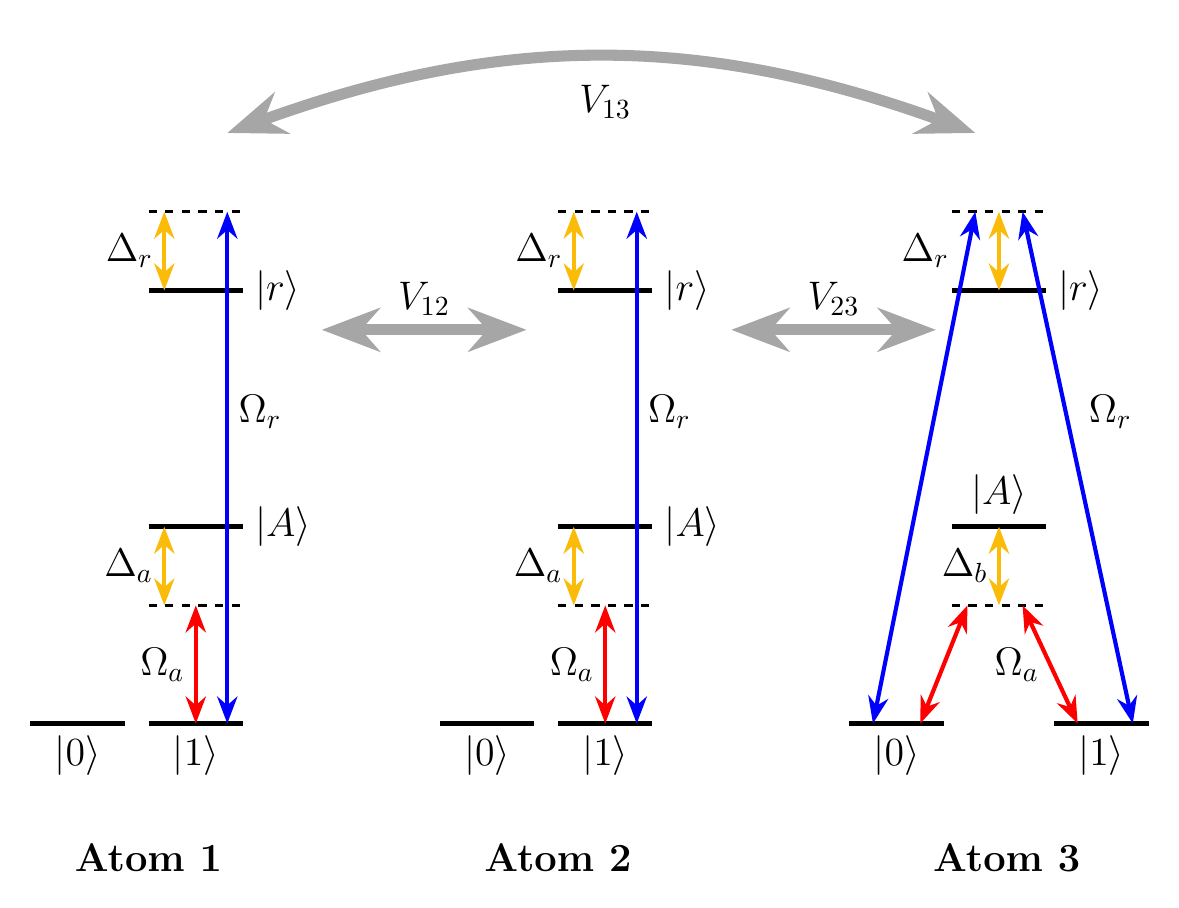
\begin{tikzpicture}[
    % ================= Styles =================
    level/.style={line width=2pt},                 % 实能级
    vlevel/.style={line width=1.2pt, dashed},         % 虚能级
    laser/.style={<->,line width=1.5pt,>=Stealth},         % 激光
    detune/.style={<->,line width=1.5pt,>=Stealth},            % 失谐 Δ
    int/.style={<->,line width=4pt,draw=gray!70,>=Stealth},
    every node/.style={font=\Large\bfseries,text=black}
]

% =========================================================
% Global geometry parameters
% =========================================================
\def\xA{0}
\def\xB{5.2}
\def\xC{10.4}

\def\yzero{0}
\def\yA{3-0.5}
\def\yr{6-0.5}

\def\yAv{2-0.5}     % |A> 虚能级
\def\yrv{7-0.5}     % |r> 虚能级

% =========================================================
% ===================== Atom 1 =============================
% =========================================================

% ----- Real levels -----
\draw[level] (\xA,\yzero) -- ++(1.2,0) node[midway,below] {$\ket{0}$};
\draw[level] (\xA+1.5,\yzero) -- ++(1.2,0) node[midway,below] {$\ket{1}$};
\draw[level] (\xA+1.5,\yA) -- ++(1.2,0) node[right] {$\ket{A}$};
\draw[level] (\xA+1.5,\yr) -- ++(1.2,0) node[right] {$\ket{r}$};

% ----- Virtual levels -----
\draw[vlevel] (\xA+1.5,\yAv) -- ++(1.2,0);
\draw[vlevel] (\xA+1.5,\yrv) -- ++(1.2,0);

% ----- Lasers -----
\draw[laser, red]
    (\xA+2.1,\yzero) -- (\xA+2.1,\yAv)
    node[midway,left] {$\Omega_a$};

\draw[laser, blue]
    (\xA+2.5,\yzero) -- (\xA+2.5,\yrv)
    node[midway,right,yshift=20px] {$\Omega_r$};

% ----- Detunings -----
\draw[detune,yellow!50!orange]
    (\xA+1.7,\yA) -- (\xA+1.7,\yAv)
    node[midway,left] {$\Delta_a$};

\draw[detune,yellow!50!orange]
    (\xA+1.7,\yr) -- (\xA+1.7,\yrv)
    node[midway,left] {$\Delta_r$};

\node at (\xA+1.5,-1.7) {Atom 1};

% =========================================================
% ===================== Atom 2 =============================
% =========================================================

\draw[level] (\xB,\yzero) -- ++(1.2,0) node[midway,below] {$\ket{0}$};
\draw[level] (\xB+1.5,\yzero) -- ++(1.2,0) node[midway,below] {$\ket{1}$};
\draw[level] (\xB+1.5,\yA) -- ++(1.2,0) node[right] {$\ket{A}$};
\draw[level] (\xB+1.5,\yr) -- ++(1.2,0) node[right] {$\ket{r}$};

% ----- Virtual levels -----
\draw[vlevel] (\xB+1.5,\yAv) -- ++(1.2,0);
\draw[vlevel] (\xB+1.5,\yrv) -- ++(1.2,0);

% ----- Lasers -----
\draw[laser, red]
    (\xB+2.1,\yzero) -- (\xB+2.1,\yAv)
    node[midway,left] {$\Omega_a$};

\draw[laser, blue]
    (\xB+2.5,\yzero) -- (\xB+2.5,\yrv)
    node[midway,right,yshift=20px] {$\Omega_r$};

% ----- Detunings -----
\draw[detune,yellow!50!orange]
    (\xB+1.7,\yA) -- (\xB+1.7,\yAv)
    node[midway,left] {$\Delta_a$};

\draw[detune,yellow!50!orange]
    (\xB+1.7,\yr) -- (\xB+1.7,\yrv)
    node[midway,left] {$\Delta_r$};

\node at (\xB+1.5,-1.7) {Atom 2};

% =========================================================
% ===================== Atom 3 (Λ) =========================
% =========================================================

% ----- Real levels -----
\draw[level] (\xC,\yzero) -- ++(1.2,0) node[midway,below] {$\ket{0}$};
\draw[level] (\xC+2.6,\yzero) -- ++(1.2,0) node[midway,below] {$\ket{1}$};
\draw[level] (\xC+1.3,\yA) -- ++(1.2,0) node[midway,above] {$\ket{A}$};
\draw[level] (\xC+1.3,\yr) -- ++(1.2,0) node[right] {$\ket{r}$};

% ----- Virtual levels -----
\draw[vlevel] (\xC+1.3,\yAv) -- ++(1.2,0);
\draw[vlevel] (\xC+1.3,\yrv) -- ++(1.2,0);

% ----- Λ lasers -----
\draw[laser, blue]
    (\xC+0.3,\yzero) -- (\xC+1.6,\yrv)
    node[midway,left] {};

\draw[laser, blue]
    (\xC+3.6,\yzero) -- (\xC+2.2,\yrv)
    node[midway,right,yshift=20px] {$\Omega_r$};

\draw[laser, red]
    (\xC+1.5,\yAv) -- (\xC+0.9,\yzero)
    node[midway,left] {};

\draw[laser, red]
    (\xC+2.2,\yAv) -- (\xC+2.9,\yzero)
    node[midway,left] {$\Omega_a$};

% ----- Detunings -----
\draw[detune,yellow!50!orange]
    (\xC+1.9,\yA) -- (\xC+1.9,\yAv)
    node[midway,left] {$\Delta_b$};

\draw[detune,yellow!50!orange]
    (\xC+1.9,\yr) -- (\xC+1.9,\yrv)
    node[midway,left,xshift=-14pt] {$\Delta_r$};

\node at (\xC+2,-1.7) {Atom 3};

% =========================================================
% ================= Rydberg interactions ===================
% =========================================================

\draw[int]
    (\xA+3.7,\yrv-1.5) -- (\xB+1.1,\yrv-1.5)
    node[midway,above] {$V_{12}$};

\draw[int]
    (\xB+3.7,\yrv-1.5) -- (\xC+1.1,\yrv-1.5)
    node[midway,above] {$V_{23}$};

\draw[int]
  (\xA+2.5,\yrv+1)
  to[out=20, in=160]
  (\xC+1.6,\yrv+1)
  node at(\xB+2.1,\yrv+1.4) {$V_{13}$};

\end{tikzpicture}

\end{document}
